\fancyhead{}
\fancyfoot{}
\cfoot{\thepage}


\lhead{Método}

\chapter{Método}

Este capítulo tiene como propósito detallar el enfoque metodológico y técnico seguido para el desarrollo del "Sistema de Asistencia Basado en Reconocimiento Facial para la FPUNE". Se presenta la planificación general del proyecto, desde la definición de los requisitos iniciales hasta la validación y evaluación del sistema implementado en un entorno académico real.

Este capítulo constituye un componente fundamental para comprender la implementación técnica del proyecto y validar su efectividad en relación con los objetivos propuestos.

En primer lugar, se describe el enfoque metodológico adoptado, el cual combina técnicas cualitativas y cuantitativas bajo un esquema de investigación aplicada tecnológica, permitiendo así un análisis integral del problema y su solución. Posteriormente, se exponen las fases específicas del proceso de desarrollo, tales como la recolección y preprocesamiento de datos, la selección de algoritmos, el entrenamiento del modelo, y la integración del sistema en un entorno controlado.


\section{Enfoque}

El presente trabajo se caracteriza por ser una investigación aplicada de tipo tecnológico, orientada al desarrollo de un sistema automatizado de control de asistencia basado en reconocimiento facial.

El enfoque de análisis de datos es mixto, combinando métodos cuantitativos y cualitativos. El primero permite medir la precisión y el rendimiento del sistema, mientras que el segundo considera la percepción de los usuarios sobre su facilidad de uso y utilidad en el entorno académico.

El alcance de la investigación es de tipo descriptivo, ya que se analizan los componentes, el funcionamiento y los resultados obtenidos durante la implementación del sistema.

El diseño de la investigación es no experimental y longitudinal, dado que el sistema será implementado y evaluado a lo largo de un semestre académico, permitiendo observar su desempeño y evolución en diferentes etapas.


\section{Método utilizado para el desarrollo}

El desarrollo de este trabajo se basó en la metodología ágil \textbf{Scrum}, la cual se centra en la planificación iterativa y la entrega progresiva de resultados funcionales. Este enfoque permite organizar el proyecto en ciclos cortos de trabajo denominados \textit{sprints}, donde se desarrollan y mejoran las distintas funcionalidades del sistema.\cite{atlassianScrum2024}

Scrum se fundamenta en los principios de transparencia, inspección y adaptación, promoviendo la colaboración y la comunicación continua entre los miembros del equipo. En este proyecto, se realizaron reuniones semanales para planificar tareas, revisar avances y establecer los objetivos del siguiente ciclo.

% ... último párrafo de "Método utilizado para el desarrollo"

\begin{figure}[H]
  \centering
  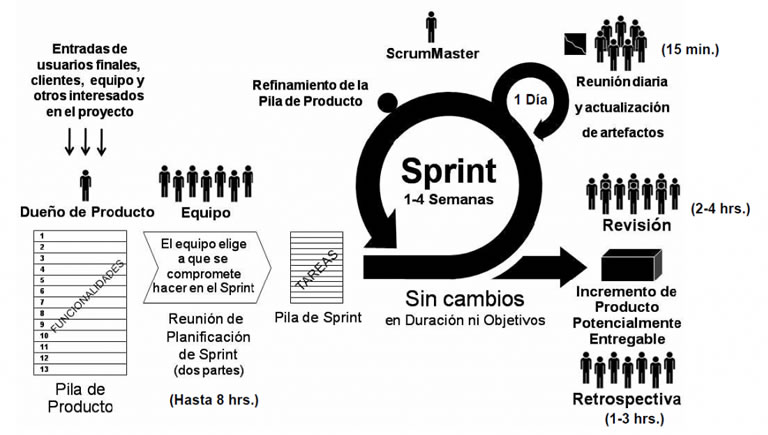
\includegraphics[width=0.99\textwidth]{imagenes_doc/Sprints.jpg}
  \caption{Ciclo de desarrollo bajo la metodología ágil Scrum.}
  \label{fig:scrum}
\end{figure}




\section{Fases del Proceso Investigativo}

\begin{itemize}
  \item \textbf{Identificación requisitos del proyecto} \\
  Se identificaron las necesidades y objetivos del sistema, considerando el número de usuarios, el entorno de aplicación, la precisión requerida y las condiciones de iluminación propias de las aulas de la FPUNE. Esta etapa permitió definir los requerimientos funcionales y no funcionales, así como los recursos técnicos necesarios para el desarrollo.

   \item \textbf{Recolección y preparación de datos} \\
  Se llevó a cabo la recopilación de imágenes faciales de los usuarios en distintas condiciones de iluminación, expresiones y ángulos, con el fin de conformar una base de datos representativa. Las imágenes fueron preprocesadas mediante normalización, eliminación de ruido y ajustes de brillo y contraste.

  \newpage
  \item \textbf{Entrenamiento del modelo} \\
  Utilizando las imágenes preprocesadas, se entrenó el modelo para generar representaciones vectoriales (embeddings) únicas de cada rostro, lo que permite su posterior comparación y verificación. Esta fase fue esencial para optimizar la precisión del reconocimiento facial.

  \item \textbf{Diseño del sistema} \\
  Se definió la arquitectura modular del sistema, integrando los componentes de captura, procesamiento, reconocimiento facial y registro en la base de datos. Además, se diseñó la base de datos relacional para almacenar tanto los datos de los usuarios como los registros de asistencia.

 
  \item \textbf{Pruebas e implementación} \\
  Se realizaron pruebas funcionales en entornos controlados para evaluar el desempeño del sistema. Posteriormente, se implementó una prueba piloto en un aula de la FPUNE, ajustando parámetros de reconocimiento para mejorar la precisión y reducir los falsos positivos.
  
\end{itemize}


\section{Análisis y selección de herramientas}

Durante esta fase se realizó un análisis comparativo de diversas tecnologías y librerías aplicadas en el desarrollo de sistemas de reconocimiento facial. La selección de herramientas se basó en criterios como precisión, rendimiento, compatibilidad, facilidad de integración y disponibilidad de documentación. 

A continuación, se detallan las principales herramientas seleccionadas:

\begin{itemize}

\item \textbf{Modelos de detección y reconocimiento facial:} \\
Se analizaron alternativas basadas en aprendizaje profundo, priorizando aquellas que ofrecen un equilibrio entre precisión y velocidad de procesamiento. Se optó por el uso de \textbf{YOLO-Face} para la detección de rostros en tiempo real, y por la librería \textbf{DeepFace} con el modelo \textbf{ArcFace} para la verificación facial, debido a su alta exactitud y estabilidad ante variaciones de iluminación, ángulo y expresión.

\item \textbf{Framework de desarrollo backend:} \\
Para la construcción de la API y la gestión de la lógica del sistema se empleó \textbf{Flask}, un microframework de Python que permite desarrollar aplicaciones ligeras y escalables. Su estructura modular facilita la integración con librerías de visión por computadora y bases de datos.

\item \textbf{Framework de desarrollo frontend:} \\
La interfaz de usuario fue desarrollada en \textbf{React}, permitiendo una interacción dinámica y fluida con el sistema. Su arquitectura basada en componentes favorece la reutilización del código y la visualización en tiempo real de los registros de asistencia.

\item \textbf{Base de datos:} \\
Se utilizó \textbf{PostgreSQL} para el almacenamiento estructurado de la información, incluyendo los registros de asistencia y datos de usuarios. Su robustez y soporte para operaciones concurrentes la convierten en una opción óptima para sistemas de este tipo.

\item \textbf{Herramienta de pruebas de API:} \\
Durante el proceso de desarrollo e integración, se empleó \textbf{Postman} para realizar pruebas de comunicación entre el frontend y el backend. Esta herramienta permitió verificar el correcto funcionamiento de las rutas, peticiones y respuestas del sistema antes de su despliegue final.

\end{itemize}

La combinación de estas herramientas permitió un desarrollo eficiente, garantizando la integración adecuada entre los módulos de detección, reconocimiento y gestión de asistencia dentro del sistema.


\section{Recolección de datos}

Para el funcionamiento del sistema de reconocimiento facial, fue necesario disponer de un conjunto de imágenes faciales representativas de los usuarios. Durante el registro de cada nuevo usuario, el sistema captura un mínimo de cinco imágenes desde diferentes ángulos y expresiones, con el fin de mejorar la capacidad de reconocimiento en distintas condiciones de uso.

Las imágenes se obtienen con cámaras externas (teléfonos móviles, webcams o cámaras digitales) y posteriormente se cargan al sistema mediante el módulo de registro de nuevos estudiantes. Durante este proceso se verifica el formato y un tamaño mínimo recomendado para preservar los rasgos faciales. Cada archivo se organiza en una carpeta individual asociada al usuario correspondiente y se nombra de forma sistemática, facilitando su identificación y el procesamiento posterior.

En la Figura~\ref{fig:rostro_original} se muestra un ejemplo de una imagen facial capturada al natural durante el proceso de registro, mientras que la Figura~\ref{fig:rostro_normalizado} presenta el resultado tras aplicar el preprocesamiento correspondiente.

\begin{figure}[H]
    \centering
    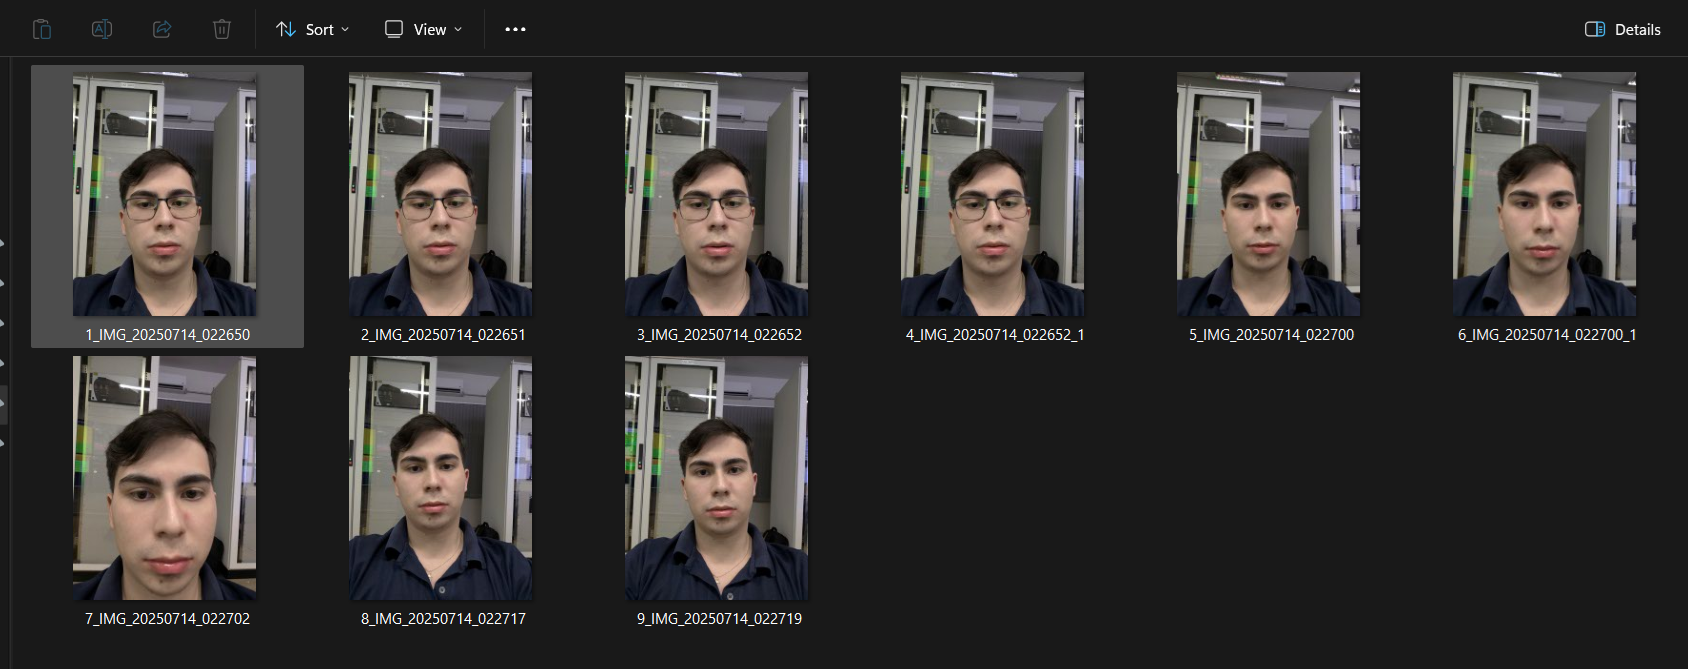
\includegraphics[width=0.99\textwidth]{imagenes_doc/sin_normalizar.png}
    \caption{Ejemplo de imagen facial capturada al natural.}
    \label{fig:rostro_original}
\end{figure}

\begin{figure}[H]
    \centering
    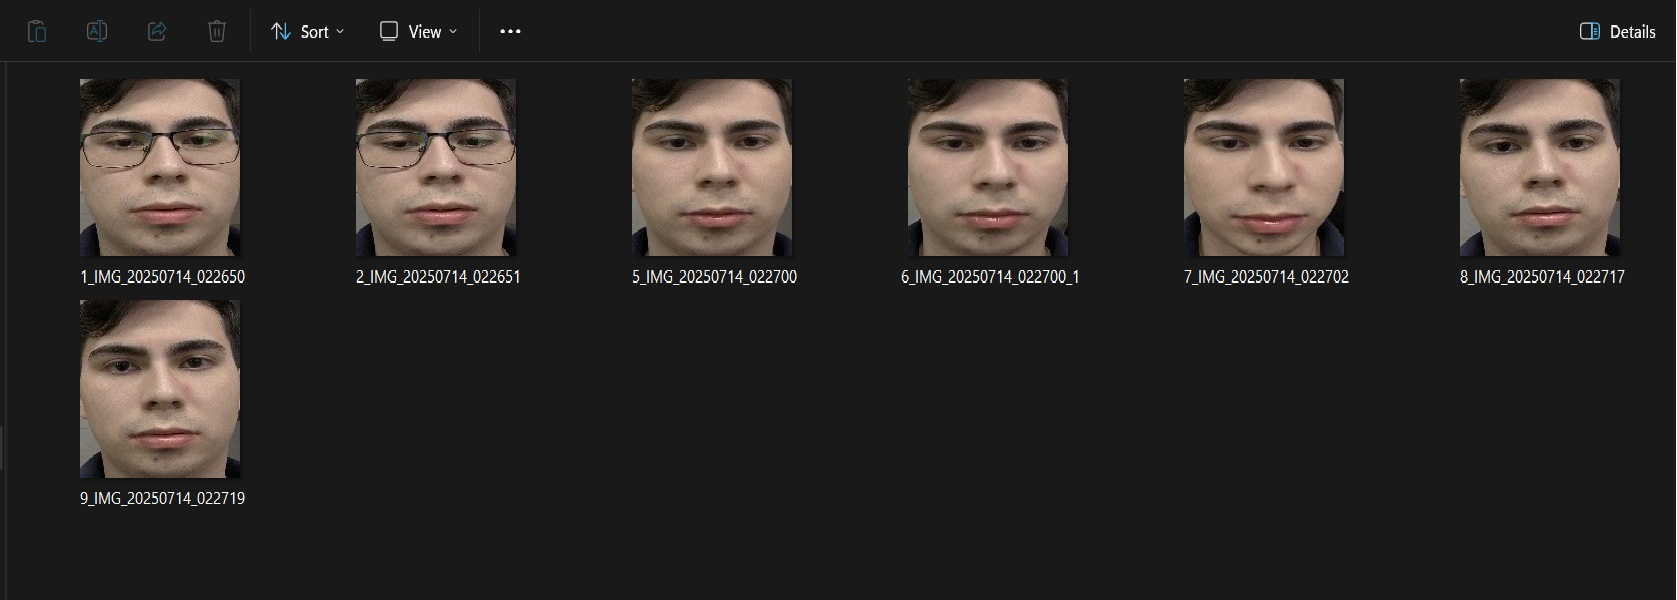
\includegraphics[width=0.99\textwidth]{imagenes_doc/dataset_rostros.jpg}
    \caption{Ejemplo de imagen facial luego del proceso de normalización.}
    \label{fig:rostro_normalizado}
\end{figure}

El proceso de preprocesamiento incluye la detección automática del rostro, recorte, alineación, y ajustes de brillo y contraste. Este procedimiento asegura que todas las imágenes presenten condiciones similares de entrada, mejorando la precisión del modelo en la identificación de los usuarios en tiempo real.


